% !TEX TS-program = pdflatex
\documentclass[11pt]{article}

% -------------------- Packages --------------------
\usepackage[a4paper,margin=1in]{geometry}
\usepackage{amsmath,amssymb}
\usepackage[T1]{fontenc}
\usepackage{lmodern}
\usepackage{xcolor}
\usepackage{tcolorbox}
\tcbuselibrary{skins,breakable}
\usepackage{enumitem}
\usepackage{hyperref}
\usepackage{tikz}
\usetikzlibrary{calc,arrows.meta}

\pagestyle{empty}

% -------------------- Dark Theme Colors --------------------
\definecolor{bg}{HTML}{000000}
\definecolor{pairbg}{HTML}{121212}
\definecolor{solbg}{HTML}{0A0A0A}
\definecolor{border}{HTML}{2A2A2A}
\definecolor{text}{HTML}{FFFFFF}
\definecolor{muted}{HTML}{C9CDD3}
\definecolor{gold}{HTML}{FFD700}
\definecolor{green}{HTML}{4ADE80}
\definecolor{cyan}{HTML}{38BDF8}

\pagecolor{bg}
\color{text}

\hypersetup{
  colorlinks=true,
  linkcolor=cyan,
  urlcolor=cyan
}

\setlength{\parindent}{0pt}
\setlength{\parskip}{10pt}

\setlist[itemize]{left=1.4em,itemsep=6pt,topsep=6pt}
\setlist[enumerate]{left=1.6em,itemsep=4pt,topsep=4pt}

% -------------------- tcolorbox Base --------------------
\tcbset{
  enhanced,
  breakable,
  arc=12pt,
  boxrule=0.8pt,
  left=16pt,right=16pt,top=12pt,bottom=12pt
}

\newtcolorbox{QAPair}[1]{%
  colback=pairbg,
  colbacklower=solbg,
  colframe=border,
  coltext=text,
  title=\textcolor{gold}{\bfseries #1},
  fonttitle=\bfseries,
  coltitle=text,
  segmentation style={draw=border, dashed, line width=0.6pt},
}

% Visible text inside this box (fix)
\newtcolorbox{QuickBox}{%
  colback=pairbg,
  colframe=cyan,
  coltext=text,
  fontupper=\color{text},
  borderline north={4pt}{0pt}{cyan},
  arc=14pt,
  boxrule=0.8pt
}

% Helper for step headings
\newcommand{\Step}[1]{\textcolor{muted}{\textbf{Step #1:}}}

% TikZ style
\tikzset{
  solidline/.style={draw=cyan, line width=0.9pt},
  dashedline/.style={draw=cyan, line width=0.9pt, dashed},
  lab/.style={text=muted, font=\small},
}

% ============================================================
\begin{document}

\begin{center}
{\LARGE\bfseries \textcolor{gold}{Exercise 9.4 --- Solutions}}\\[-2pt]
\end{center}

\begin{QuickBox}
{\color{cyan}\bfseries Quick formulas (Similarity of Solids)}\par\medskip
\begin{itemize}
\item If two solids are \textbf{similar} and the \textbf{linear scale factor} is $k$ (e.g., $\text{small}:\text{large}=k:1$), then:
\[
\frac{\text{Surface Areas}}{}:\; k^2,\qquad
\frac{\text{Volumes}}{}:\; k^3.
\]
\item From \textbf{surface area ratio} $\dfrac{S_1}{S_2}$, the linear scale factor is $k=\sqrt{\dfrac{S_1}{S_2}}$.
\item From \textbf{volume ratio} $\dfrac{V_1}{V_2}$, the linear scale factor is $k=\sqrt[3]{\dfrac{V_1}{V_2}}$.
\item Useful volumes: Cylinder $V=\pi r^2 h$, Cone $V=\dfrac13\pi r^2 h$, Pyramid $V=\dfrac13(\text{base area})\cdot h$.
\end{itemize}
\end{QuickBox}

% ============================================================
% Q1
\begin{QAPair}{Question 1 (i)}
\textcolor{gold}{\bfseries Question:} Determine whether the two cuboids are similar or not.\\[4pt]
\begin{center}
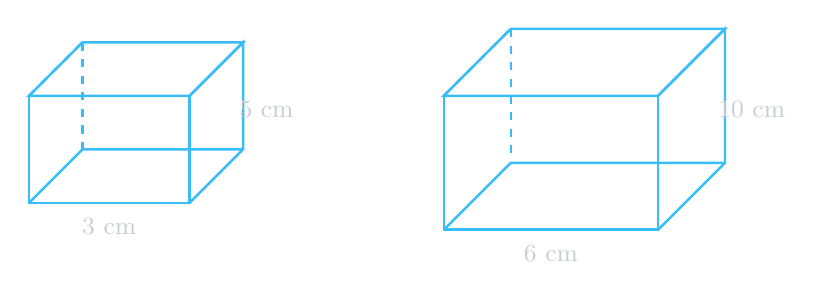
\begin{tikzpicture}[scale=0.85]
% small cuboid
\draw[solidline] (0,0) -- (2.4,0) -- (3.2,0.8) -- (0.8,0.8) -- cycle;
\draw[solidline] (0,0) -- (0,-1.6) -- (2.4,-1.6) -- (2.4,0);
\draw[solidline] (2.4,0) -- (3.2,0.8) -- (3.2,-0.8) -- (2.4,-1.6);
\draw[solidline] (0,-1.6) -- (0.8,-0.8) -- (3.2,-0.8);
\draw[dashedline] (0,0) -- (0.8,0.8);
\draw[dashedline] (0.8,0.8) -- (0.8,-0.8);
\node[lab] at (1.2,-1.95) {$3\text{ cm}$};
\node[lab] at (3.55,-0.2) {$5\text{ cm}$};

% large cuboid
\begin{scope}[xshift=6.2cm]
\draw[solidline] (0,0) -- (3.2,0) -- (4.2,1.0) -- (1.0,1.0) -- cycle;
\draw[solidline] (0,0) -- (0,-2.0) -- (3.2,-2.0) -- (3.2,0);
\draw[solidline] (3.2,0) -- (4.2,1.0) -- (4.2,-1.0) -- (3.2,-2.0);
\draw[solidline] (0,-2.0) -- (1.0,-1.0) -- (4.2,-1.0);
\draw[dashedline] (0,0) -- (1.0,1.0);
\draw[dashedline] (1.0,1.0) -- (1.0,-1.0);
\node[lab] at (1.6,-2.35) {$6\text{ cm}$};
\node[lab] at (4.6,-0.2) {$10\text{ cm}$};
\end{scope}
\end{tikzpicture}
\end{center}
\tcblower
\textcolor{green}{\bfseries Answer:}
\[
\begin{aligned}
\Step{1}\;& \text{Compare corresponding lengths: } \frac{3}{6}=\frac{1}{2},\quad \frac{5}{10}=\frac{1}{2}.\\
\Step{2}\;& \text{Both given ratios are equal, so the solids are similar.}\\
\Step{3}\;& \text{Scale factor (small : large)}=1:2.
\end{aligned}
\]
\end{QAPair}

\begin{QAPair}{Question 1 (ii)}
\textcolor{gold}{\bfseries Question:} Determine whether the two cylinders are similar or not.\\[4pt]
\begin{center}
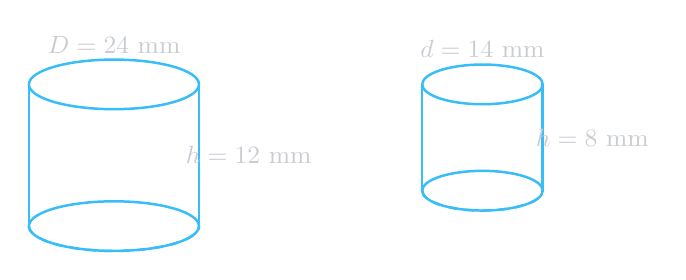
\begin{tikzpicture}[scale=0.9]
% Cylinder 1
\draw[solidline] (0,0) ellipse (1.2 and 0.35);
\draw[solidline] (-1.2,0) -- (-1.2,-2.0);
\draw[solidline] (1.2,0) -- (1.2,-2.0);
\draw[solidline] (0,-2.0) ellipse (1.2 and 0.35);
\draw[dashedline] (-1.2,-2.0) arc (180:360:1.2 and 0.35);
\node[lab] at (0,0.55) {$D=24\text{ mm}$};
\node[lab] at (1.9,-1.0) {$h=12\text{ mm}$};

% Cylinder 2
\begin{scope}[xshift=5.2cm]
\draw[solidline] (0,0) ellipse (0.85 and 0.28);
\draw[solidline] (-0.85,0) -- (-0.85,-1.5);
\draw[solidline] (0.85,0) -- (0.85,-1.5);
\draw[solidline] (0,-1.5) ellipse (0.85 and 0.28);
\draw[dashedline] (-0.85,-1.5) arc (180:360:0.85 and 0.28);
\node[lab] at (0,0.5) {$d=14\text{ mm}$};
\node[lab] at (1.55,-0.75) {$h=8\text{ mm}$};
\end{scope}
\end{tikzpicture}
\end{center}
\tcblower
\textcolor{green}{\bfseries Answer:}
\[
\begin{aligned}
\Step{1}\;& \text{For similarity, } \frac{D_1}{D_2}=\frac{h_1}{h_2}.\\
\Step{2}\;& \frac{24}{14}=\frac{12}{7}\neq \frac{12}{8}=\frac{3}{2}.\\
\Step{3}\;& \Rightarrow \textbf{Not similar.}
\end{aligned}
\]
\end{QAPair}

\begin{QAPair}{Question 1 (iii)}
\textcolor{gold}{\bfseries Question:} Determine whether the two pyramids are similar or not.\\[4pt]
\begin{center}
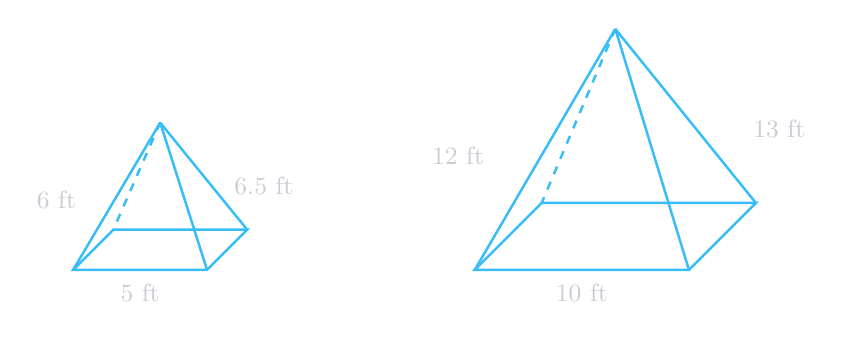
\begin{tikzpicture}[scale=0.85]
% small pyramid
\draw[solidline] (0,0) -- (2,0) -- (2.6,0.6) -- (0.6,0.6) -- cycle;
\draw[solidline] (1.3,2.2) -- (0,0);
\draw[solidline] (1.3,2.2) -- (2,0);
\draw[solidline] (1.3,2.2) -- (2.6,0.6);
\draw[dashedline] (1.3,2.2) -- (0.6,0.6);
\node[lab] at (1,-0.35) {$5\text{ ft}$};
\node[lab] at (-0.25,1.05) {$6\text{ ft}$};
\node[lab] at (2.85,1.25) {$6.5\text{ ft}$};

% large pyramid
\begin{scope}[xshift=6.0cm]
\draw[solidline] (0,0) -- (3.2,0) -- (4.2,1.0) -- (1.0,1.0) -- cycle;
\draw[solidline] (2.1,3.6) -- (0,0);
\draw[solidline] (2.1,3.6) -- (3.2,0);
\draw[solidline] (2.1,3.6) -- (4.2,1.0);
\draw[dashedline] (2.1,3.6) -- (1.0,1.0);
\node[lab] at (1.6,-0.35) {$10\text{ ft}$};
\node[lab] at (-0.25,1.7) {$12\text{ ft}$};
\node[lab] at (4.55,2.1) {$13\text{ ft}$};
\end{scope}
\end{tikzpicture}
\end{center}
\tcblower
\textcolor{green}{\bfseries Answer:}
\[
\begin{aligned}
\Step{1}\;& \frac{5}{10}=\frac{1}{2},\quad \frac{6}{12}=\frac{1}{2},\quad \frac{6.5}{13}=\frac{1}{2}.\\
\Step{2}\;& \text{All corresponding lengths are in the same ratio.}\\
\Step{3}\;& \Rightarrow \textbf{Similar}, \text{ scale factor (small : large)}=1:2.
\end{aligned}
\]
\end{QAPair}

\begin{QAPair}{Question 1 (iv)}
\textcolor{gold}{\bfseries Question:} Determine whether the two cones are similar or not.\\[4pt]
\begin{center}
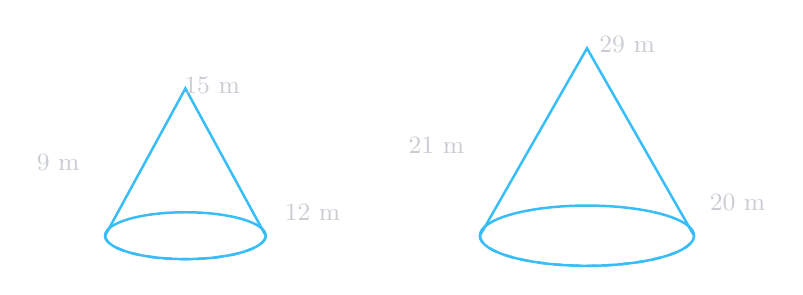
\begin{tikzpicture}[scale=0.85]
% small cone
\draw[solidline] (0,0) ellipse (1.2 and 0.35);
\draw[solidline] (-1.2,0) -- (0,2.2) -- (1.2,0);
\draw[dashedline] (-1.2,0) arc (180:360:1.2 and 0.35);
\node[lab] at (-1.9,1.1) {$9\text{ m}$};
\node[lab] at (1.9,0.35) {$12\text{ m}$};
\node[lab] at (0.4,2.25) {$15\text{ m}$};

% large cone
\begin{scope}[xshift=6.0cm]
\draw[solidline] (0,0) ellipse (1.6 and 0.45);
\draw[solidline] (-1.6,0) -- (0,2.8) -- (1.6,0);
\draw[dashedline] (-1.6,0) arc (180:360:1.6 and 0.45);
\node[lab] at (-2.25,1.35) {$21\text{ m}$};
\node[lab] at (2.25,0.5) {$20\text{ m}$};
\node[lab] at (0.6,2.85) {$29\text{ m}$};
\end{scope}
\end{tikzpicture}
\end{center}
\tcblower
\textcolor{green}{\bfseries Answer:}
\[
\begin{aligned}
\Step{1}\;& \text{Compare ratios: } \frac{9}{20}\neq \frac{12}{21}\neq \frac{15}{29}.\\
\Step{2}\;& \text{Corresponding lengths are not proportional.}\\
\Step{3}\;& \Rightarrow \textbf{Not similar.}
\end{aligned}
\]
\end{QAPair}

% ============================================================
% Q2
\begin{QAPair}{Question 2 (i)}
\textcolor{gold}{\bfseries Question:} Solids are similar. Find the unknown and also the ratio of volumes.\\
Big cylinder: $D=100\text{ m},\; H=25\text{ m}$;\quad Small cylinder: $d=?,\; h=5\text{ m}$.\\[4pt]
\begin{center}
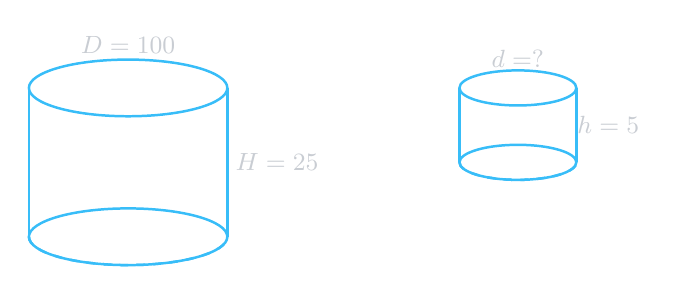
\begin{tikzpicture}[scale=0.9]
\draw[solidline] (0,0) ellipse (1.4 and 0.4);
\draw[solidline] (-1.4,0) -- (-1.4,-2.1);
\draw[solidline] (1.4,0) -- (1.4,-2.1);
\draw[solidline] (0,-2.1) ellipse (1.4 and 0.4);
\draw[dashedline] (-1.4,-2.1) arc (180:360:1.4 and 0.4);
\node[lab] at (0,0.6) {$D=100$};
\node[lab] at (2.1,-1.05) {$H=25$};

\begin{scope}[xshift=5.5cm,scale=0.75]
\draw[solidline] (0,0) ellipse (1.1 and 0.33);
\draw[solidline] (-1.1,0) -- (-1.1,-1.4);
\draw[solidline] (1.1,0) -- (1.1,-1.4);
\draw[solidline] (0,-1.4) ellipse (1.1 and 0.33);
\draw[dashedline] (-1.1,-1.4) arc (180:360:1.1 and 0.33);
\node[lab] at (0,0.55) {$d=?$};
\node[lab] at (1.7,-0.7) {$h=5$};
\end{scope}
\end{tikzpicture}
\end{center}
\tcblower
\textcolor{green}{\bfseries Answer:}
\[
\begin{aligned}
\Step{1}\;& \text{Linear scale factor (big : small)}=\frac{H}{h}=\frac{25}{5}=5:1.\\
\Step{2}\;& \frac{D}{d}=5 \;\Rightarrow\; d=\frac{100}{5}=20\text{ m}.\\
\Step{3}\;& \text{Volume ratio (big : small)}=5^3:1^3=125:1.
\end{aligned}
\]
\end{QAPair}

\begin{QAPair}{Question 2 (ii)}
\textcolor{gold}{\bfseries Question:} Solids are similar. Find the values of $b,c,h$ and also the ratio of volumes.\\
(Smaller solid has a right-triangle face with sides $5\text{ m}$, $c$, and hypotenuse $13\text{ m}$, and length $6\text{ m}$.)\\[4pt]
\begin{center}
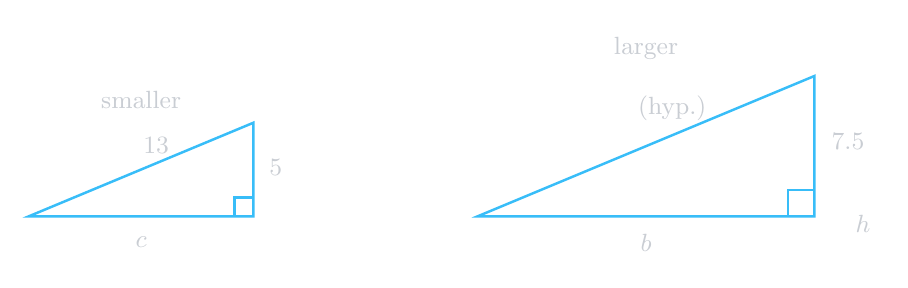
\begin{tikzpicture}[scale=0.95]
% small right triangle (5-12-13)
\draw[solidline] (0,0) -- (3,0) -- (3,1.25) -- cycle;
\draw[solidline] (2.75,0) -- (2.75,0.25) -- (3,0.25);
\node[lab] at (1.5,-0.35) {$c$};
\node[lab] at (3.3,0.65) {$5$};
\node[lab] at (1.7,0.95) {$13$};
\node[lab] at (1.5,1.55) {\small smaller};

% large right triangle scaled (7.5,18,19.5)
\begin{scope}[xshift=6.0cm]
\draw[solidline] (0,0) -- (4.5,0) -- (4.5,1.875) -- cycle;
\draw[solidline] (4.15,0) -- (4.15,0.35) -- (4.5,0.35);
\node[lab] at (2.25,-0.35) {$b$};
\node[lab] at (4.95,1.0) {$7.5$};
\node[lab] at (2.6,1.45) {$\text{(hyp.)}$};
\node[lab] at (2.25,2.25) {\small larger};
\node[lab] at (5.15,-0.1) {$h$};
\end{scope}
\end{tikzpicture}
\end{center}
\tcblower
\textcolor{green}{\bfseries Answer:}
\[
\begin{aligned}
\Step{1}\;& \text{In the small right triangle: } 5^2+c^2=13^2\\
&\Rightarrow c^2=169-25=144 \Rightarrow c=12\text{ m}.\\[4pt]
\Step{2}\;& \text{Scale factor (larger : smaller)}=\frac{7.5}{5}=\frac{3}{2}.\\
\Step{3}\;& b=12\cdot \frac{3}{2}=18\text{ m},\qquad h=6\cdot \frac{3}{2}=9\text{ m}.\\
\Step{4}\;& \text{Volume ratio (larger : smaller)}=\left(\frac{3}{2}\right)^3=\frac{27}{8}\Rightarrow 27:8.
\end{aligned}
\]
\end{QAPair}

% ============================================================
% Q3
\begin{QAPair}{Question 3 (i)}
\textcolor{gold}{\bfseries Question:} Solids are similar. Find $V_2$.\\
Big pyramid: side $21\text{ mm}$, $V_1=9000\text{ mm}^3$;\quad Small pyramid: side $7\text{ mm}$.
\tcblower
\textcolor{green}{\bfseries Answer:}
\[
\begin{aligned}
\Step{1}\;& \text{Linear ratio (small : big)}=\frac{7}{21}=\frac{1}{3}.\\
\Step{2}\;& \text{Volume ratio}=\left(\frac{1}{3}\right)^3=\frac{1}{27}.\\
\Step{3}\;& V_2=9000\cdot \frac{1}{27}=\frac{9000}{27}=\frac{1000}{3}\text{ mm}^3
=333\tfrac{1}{3}\text{ mm}^3.
\end{aligned}
\]
\end{QAPair}

\begin{QAPair}{Question 3 (ii)}
\textcolor{gold}{\bfseries Question:} Cylinders are similar. Big cylinder has radius $12\text{ ft}$ and $V_2=360\text{ ft}^3$. Small cylinder has radius $10\text{ ft}$. Find $V_1$.
\tcblower
\textcolor{green}{\bfseries Answer:}
\[
\begin{aligned}
\Step{1}\;& \text{Linear ratio (small : big)}=\frac{10}{12}=\frac{5}{6}.\\
\Step{2}\;& \text{Volume ratio}=\left(\frac{5}{6}\right)^3=\frac{125}{216}.\\
\Step{3}\;& V_1=360\cdot \frac{125}{216}
=\left(\frac{360}{216}\right)125
=\left(\frac{5}{3}\right)125
=\frac{625}{3}\text{ ft}^3\\
&=208\tfrac{1}{3}\text{ ft}^3.
\end{aligned}
\]
\end{QAPair}

\begin{QAPair}{Question 3 (iii)}
\textcolor{gold}{\bfseries Question:} Cones are similar. Small cone has slant length $6\text{ cm}$. Big cone has slant length $15\text{ cm}$ and $V_2=460\text{ cm}^3$. Find $V_1$.
\tcblower
\textcolor{green}{\bfseries Answer:}
\[
\begin{aligned}
\Step{1}\;& \text{Linear ratio (small : big)}=\frac{6}{15}=\frac{2}{5}.\\
\Step{2}\;& \text{Volume ratio}=\left(\frac{2}{5}\right)^3=\frac{8}{125}.\\
\Step{3}\;& V_1=460\cdot \frac{8}{125}=\frac{3680}{125}=29.44\text{ cm}^3.
\end{aligned}
\]
\end{QAPair}

\begin{QAPair}{Question 3 (iv)}
\textcolor{gold}{\bfseries Question:} Similar solids have a corresponding length $12\text{ m}$ for solid 1 and $9\text{ m}$ for solid 2. Given $V_1=288\text{ m}^3$, find $V_2$.
\tcblower
\textcolor{green}{\bfseries Answer:}
\[
\begin{aligned}
\Step{1}\;& \text{Linear ratio (2 : 1)}=\frac{9}{12}=\frac{3}{4}.\\
\Step{2}\;& \text{Volume ratio}=\left(\frac{3}{4}\right)^3=\frac{27}{64}.\\
\Step{3}\;& V_2=288\cdot \frac{27}{64}
=\left(\frac{288}{64}\right)27
=4.5\times 27
=121.5\text{ m}^3\\
&=\frac{243}{2}\text{ m}^3.
\end{aligned}
\]
\end{QAPair}

% ============================================================
% Q4
\begin{QAPair}{Question 4}
\textcolor{gold}{\bfseries Question:} Find the ratio of scale factors of the two similar solids with volumes $512\text{ m}^3$ and $1728\text{ m}^3$.\\[4pt]
\begin{center}
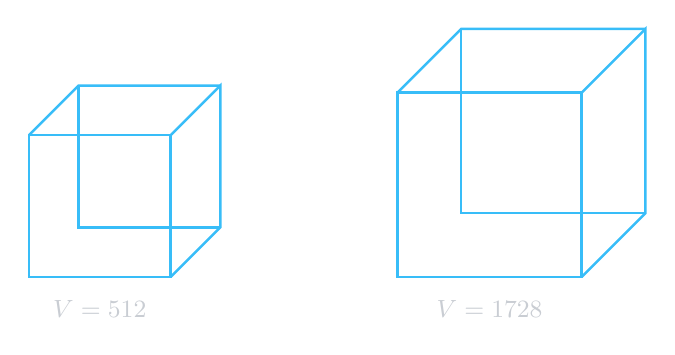
\begin{tikzpicture}[scale=0.9]
\draw[solidline] (0,0) rectangle (2,2);
\draw[solidline] (2,0) -- (2.7,0.7) -- (2.7,2.7) -- (2,2);
\draw[solidline] (0,2) -- (0.7,2.7) -- (2.7,2.7);
\draw[solidline] (0.7,2.7) -- (0.7,0.7) -- (2.7,0.7);
\node[lab] at (1,-0.45) {$V=512$};

\begin{scope}[xshift=5.2cm]
\draw[solidline] (0,0) rectangle (2.6,2.6);
\draw[solidline] (2.6,0) -- (3.5,0.9) -- (3.5,3.5) -- (2.6,2.6);
\draw[solidline] (0,2.6) -- (0.9,3.5) -- (3.5,3.5);
\draw[solidline] (0.9,3.5) -- (0.9,0.9) -- (3.5,0.9);
\node[lab] at (1.3,-0.45) {$V=1728$};
\end{scope}
\end{tikzpicture}
\end{center}
\tcblower
\textcolor{green}{\bfseries Answer:}
\[
\begin{aligned}
\Step{1}\;& \text{Linear scale factor}=\sqrt[3]{\frac{512}{1728}}
=\sqrt[3]{\frac{8^3}{12^3}}=\frac{8}{12}.\\
\Step{2}\;& \Rightarrow \text{Ratio of scale factors (smaller : larger)}=8:12=2:3.
\end{aligned}
\]
\end{QAPair}

% ============================================================
% Q5
\begin{QAPair}{Question 5}
\textcolor{gold}{\bfseries Question:} Two swimming pools are similar with scale factor $4:5$. Chlorine needed is proportional to volume. If $3$ cups are needed for the smaller pool, how much is needed for the larger pool?
\tcblower
\textcolor{green}{\bfseries Answer:}
\[
\begin{aligned}
\Step{1}\;& \text{Linear ratio (small : large)}=4:5 \Rightarrow \text{volume ratio} =4^3:5^3=64:125.\\
\Step{2}\;& \text{So } \frac{\text{large}}{\text{small}}=\frac{125}{64}.\\
\Step{3}\;& \text{Chlorine for large} = 3\cdot \frac{125}{64}=\frac{375}{64}
=5\tfrac{55}{64}\approx 5.86\text{ cups}.
\end{aligned}
\]
\end{QAPair}

% ============================================================
% Q6
\begin{QAPair}{Question 6}
\textcolor{gold}{\bfseries Question:} A model bus is built with a scale of $1:10$. The model bus has volume $30\text{ m}^3$. What is the volume of the actual bus?
\tcblower
\textcolor{green}{\bfseries Answer:}
\[
\begin{aligned}
\Step{1}\;& \text{Linear scale factor (model : actual)}=1:10.\\
\Step{2}\;& \text{Volume scale factor}=1^3:10^3=1:1000.\\
\Step{3}\;& V_{\text{actual}}=30\times 1000=30000\text{ m}^3.
\end{aligned}
\]
\end{QAPair}

% ============================================================
% Q7
\begin{QAPair}{Question 7}
\textcolor{gold}{\bfseries Question:} Solid A is similar to solid B with scale factor $2:3$. If surface area and volume of solid A are $130\pi\text{ cm}^2$ and $280\pi\text{ cm}^3$ respectively, find the surface area and volume of solid B.\\[4pt]
\begin{center}
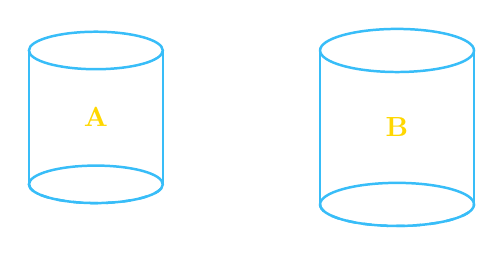
\begin{tikzpicture}[scale=0.85]
\draw[solidline] (0,0) ellipse (1.0 and 0.28);
\draw[solidline] (-1.0,0) -- (-1.0,-2.0);
\draw[solidline] (1.0,0) -- (1.0,-2.0);
\draw[solidline] (0,-2.0) ellipse (1.0 and 0.28);
\draw[dashedline] (-1.0,-2.0) arc (180:360:1.0 and 0.28);
\node[text=gold,font=\bfseries] at (0,-1.0) {A};

\begin{scope}[xshift=4.5cm,scale=1.15]
\draw[solidline] (0,0) ellipse (1.0 and 0.28);
\draw[solidline] (-1.0,0) -- (-1.0,-2.0);
\draw[solidline] (1.0,0) -- (1.0,-2.0);
\draw[solidline] (0,-2.0) ellipse (1.0 and 0.28);
\draw[dashedline] (-1.0,-2.0) arc (180:360:1.0 and 0.28);
\node[text=gold,font=\bfseries] at (0,-1.0) {B};
\end{scope}
\end{tikzpicture}
\end{center}
\tcblower
\textcolor{green}{\bfseries Answer:}
\[
\begin{aligned}
\Step{1}\;& \text{Linear ratio (A : B)}=2:3 \Rightarrow \text{(B/A)}=\frac{3}{2}.\\
\Step{2}\;& S_B=S_A\left(\frac{3}{2}\right)^2=130\pi\cdot \frac{9}{4}=\frac{1170}{4}\pi=\frac{585}{2}\pi\text{ cm}^2.\\
\Step{3}\;& V_B=V_A\left(\frac{3}{2}\right)^3=280\pi\cdot \frac{27}{8}
=35\cdot 27\,\pi=945\pi\text{ cm}^3.
\end{aligned}
\]
\end{QAPair}

% ============================================================
% Q8
\begin{QAPair}{Question 8}
\textcolor{gold}{\bfseries Question:} Solid I is similar to Solid II. Given $V_I=8\pi\text{ ft}^3$ and $V_{II}=125\pi\text{ ft}^3$, find the scale factor of solid I to solid II.\\[4pt]
\begin{center}
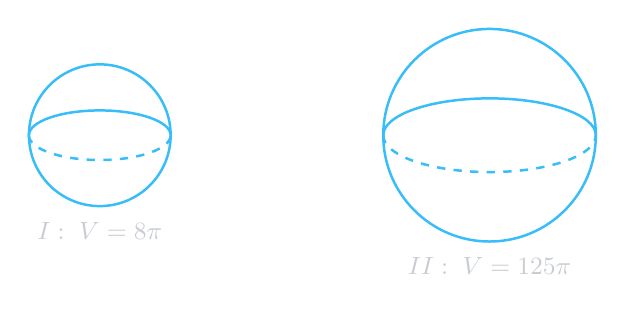
\begin{tikzpicture}[scale=0.9]
\draw[solidline] (0,0) circle (1.0);
\draw[dashedline] (-1,0) arc (180:360:1 and 0.35);
\draw[solidline] (1,0) arc (0:180:1 and 0.35);
\node[lab] at (0,-1.35) {$I:\;V=8\pi$};

\begin{scope}[xshift=5.5cm]
\draw[solidline] (0,0) circle (1.5);
\draw[dashedline] (-1.5,0) arc (180:360:1.5 and 0.52);
\draw[solidline] (1.5,0) arc (0:180:1.5 and 0.52);
\node[lab] at (0,-1.85) {$II:\;V=125\pi$};
\end{scope}
\end{tikzpicture}
\end{center}
\tcblower
\textcolor{green}{\bfseries Answer:}
\[
\begin{aligned}
\Step{1}\;& \frac{V_I}{V_{II}}=\frac{8\pi}{125\pi}=\frac{8}{125}.\\
\Step{2}\;& \text{Scale factor (I : II)}=\sqrt[3]{\frac{8}{125}}=\frac{2}{5}.\\
\Step{3}\;& \Rightarrow \boxed{2:5}.
\end{aligned}
\]
\end{QAPair}

% ============================================================
% Q9
\begin{QAPair}{Question 9}
\textcolor{gold}{\bfseries Question:} Solid A and solid B are similar. $V_A=32\text{ cm}^3$, $V_B=108\text{ cm}^3$, and height of A is $10\text{ cm}$. Find the height of B.
\tcblower
\textcolor{green}{\bfseries Answer:}
\[
\begin{aligned}
\Step{1}\;& \frac{V_B}{V_A}=\frac{108}{32}=\frac{27}{8}.\\
\Step{2}\;& \text{Linear ratio (B : A)}=\sqrt[3]{\frac{27}{8}}=\frac{3}{2}.\\
\Step{3}\;& h_B=10\cdot \frac{3}{2}=15\text{ cm}.
\end{aligned}
\]
\end{QAPair}

% ============================================================
% Q10
\begin{QAPair}{Question 10}
\textcolor{gold}{\bfseries Question:} P and Q are similar solids. Solid P has surface area $108\text{ cm}^2$ and volume $135\text{ cm}^3$. Find volume of Q if Q has surface area $300\text{ cm}^2$.
\tcblower
\textcolor{green}{\bfseries Answer:}
\[
\begin{aligned}
\Step{1}\;& \frac{S_Q}{S_P}=\frac{300}{108}=\frac{25}{9}.\\
\Step{2}\;& \text{Linear ratio (Q : P)}=\sqrt{\frac{25}{9}}=\frac{5}{3}.\\
\Step{3}\;& \frac{V_Q}{V_P}=\left(\frac{5}{3}\right)^3=\frac{125}{27}.\\
\Step{4}\;& V_Q=135\cdot \frac{125}{27}=\left(\frac{135}{27}\right)125=5\cdot 125=625\text{ cm}^3.
\end{aligned}
\]
\end{QAPair}

% ============================================================
% Q11
\begin{QAPair}{Question 11 (i)}
\textcolor{gold}{\bfseries Question:} X and Y are similar cylinders with base area ratio $16:25$. Find the ratio of heights.
\tcblower
\textcolor{green}{\bfseries Answer:}
\[
\begin{aligned}
\Step{1}\;& \text{Base area ratio}=\frac{\pi r_X^2}{\pi r_Y^2}=\frac{16}{25}.\\
\Step{2}\;& \Rightarrow \frac{r_X}{r_Y}=\sqrt{\frac{16}{25}}=\frac{4}{5}.\\
\Step{3}\;& \text{For similar cylinders, } \frac{h_X}{h_Y}=\frac{4}{5}\Rightarrow \boxed{4:5}.
\end{aligned}
\]
\end{QAPair}

\begin{QAPair}{Question 11 (ii)}
\textcolor{gold}{\bfseries Question:} X and Y are similar cylinders with base area ratio $16:25$. Find the ratio of curved surface areas.
\tcblower
\textcolor{green}{\bfseries Answer:}
\[
\begin{aligned}
\Step{1}\;& \text{Curved surface area }=2\pi r h \;\;\Rightarrow\;\; \text{scales as } k^2.\\
\Step{2}\;& \text{Since } k=\frac{4}{5},\; \text{CSA ratio }=\left(\frac{4}{5}\right)^2=\frac{16}{25}.\\
\Step{3}\;& \Rightarrow \boxed{16:25}.
\end{aligned}
\]
\end{QAPair}

\begin{QAPair}{Question 11 (iii)}
\textcolor{gold}{\bfseries Question:} X and Y are similar cylinders with base area ratio $16:25$. Find the ratio of volumes.
\tcblower
\textcolor{green}{\bfseries Answer:}
\[
\begin{aligned}
\Step{1}\;& \text{Linear ratio } k=\frac{4}{5}.\\
\Step{2}\;& \text{Volume ratio}=\left(\frac{4}{5}\right)^3=\frac{64}{125}.\\
\Step{3}\;& \Rightarrow \boxed{64:125}.
\end{aligned}
\]
\end{QAPair}

% ============================================================
% Q12
\begin{QAPair}{Question 12}
\textcolor{gold}{\bfseries Question:} The volume of one right circular cone is $8$ times the other. If the radius of the larger cone is $12\text{ cm}$, find the radius of the smaller cone.
\tcblower
\textcolor{green}{\bfseries Answer:}
\[
\begin{aligned}
\Step{1}\;& \frac{V_L}{V_S}=8=\left(\frac{r_L}{r_S}\right)^3 \quad (\text{similar cones}).\\
\Step{2}\;& \Rightarrow \frac{r_L}{r_S}=\sqrt[3]{8}=2.\\
\Step{3}\;& r_S=\frac{12}{2}=6\text{ cm}.
\end{aligned}
\]
\end{QAPair}

% ============================================================
% Q13
\begin{QAPair}{Question 13}
\textcolor{gold}{\bfseries Question:} Masses of two similar objects are $8\text{ kg}$ and $27\text{ kg}$ respectively. If the height of the first object is $2\text{ m}$, what is the height of the second object?
\tcblower
\textcolor{green}{\bfseries Answer:}
\[
\begin{aligned}
\Step{1}\;& \text{For similar objects (same material), } \frac{m_1}{m_2}=\frac{V_1}{V_2}.\\
\Step{2}\;& \frac{V_1}{V_2}=\frac{8}{27}\Rightarrow \text{linear ratio } \frac{h_1}{h_2}=\sqrt[3]{\frac{8}{27}}=\frac{2}{3}.\\
\Step{3}\;& \frac{2}{h_2}=\frac{2}{3}\Rightarrow h_2=3\text{ m}.
\end{aligned}
\]
\end{QAPair}

\end{document}
